% !TEX TS-program = xelatex
% !TEX encoding = UTF-8 Unicode
% !Mode:: "TeX:UTF-8"

%This file contains the LaTeX code of my laboratory report for my ICS II course.
%Author: 张作柏/Zuobai Zhang <17300240035@fudan.edu.cn>

% This is a simple template for a LaTeX document using the "article" class.
% See "book", "report", "letter" for other types of document.

\documentclass[12pt]{article} % use larger type; default would be 10pt

\usepackage[utf8]{inputenc} % set input encoding (not needed with XeLaTeX)

%%% Examples of Article customizations
% These packages are optional, depending whether you want the features they provide.
% See the LaTeX Companion or other references for full information.

%%% PAGE DIMENSIONS
\usepackage[top=1.05in, bottom=0.95in, left=0.90in, right=1.10in]{geometry}
%\usepackage{geometry} % to change the page dimensions
\geometry{a4paper} % or letterpaper (US) or a5paper or....
% \geometry{margin=2in} % for example, change the margins to 2 inches all round
% \geometry{landscape} % set up the page for landscape
%   read geometry.pdf for detailed page layout information

\usepackage{graphicx} % support the \includegraphics command and options

% \usepackage[parfill]{parskip} % Activate to begin paragraphs with an empty line rather than an indent

%%% PACKAGES
\usepackage{booktabs} % for much better looking tables
\usepackage{array} % for better arrays (eg matrices) in maths
\usepackage{paralist} % very flexible & customisable lists (eg. enumerate/itemize, etc.)
\usepackage{verbatim} % adds environment for commenting out blocks of text & for better verbatim
\usepackage{subfig} % make it possible to include more than one captioned figure/table in a single float
% These packages are all incorporated in the memoir class to one degree or another...

%%% HEADERS & FOOTERS
\usepackage{fancyhdr} % This should be set AFTER setting up the page geometry
\pagestyle{fancy} % options: empty , plain , fancy
%\renewcommand{\headrulewidth}{0pt} % customise the layout...
\lhead{}\chead{}\rhead{}
\lfoot{}\cfoot{\thepage}\rfoot{}

%%% SECTION TITLE APPEARANCE
\usepackage{sectsty}
\allsectionsfont{\sffamily\mdseries\upshape} % (See the fntguide.pdf for font help)
% (This matches ConTeXt defaults)

%%% ToC (table of contents) APPEARANCE
\usepackage[nottoc,notlof,notlot]{tocbibind} % Put the bibliography in the ToC
\usepackage[titles,subfigure]{tocloft} % Alter the style of the Table of Contents
\renewcommand{\cftsecfont}{\rmfamily\mdseries\upshape}
\renewcommand{\cftsecpagefont}{\rmfamily\mdseries\upshape} % No bold!
\usepackage{titletoc}
\titlecontents{section}
              [1.5cm]
              {\bf \large}%
              {\contentslabel{1.8em}}%
              {}%
              {\titlerule*[0.5pc]{$\cdot$}\contentspage\hspace*{0.6cm}}%
		   [\vspace{0.5em}]
\titlecontents{subsection}
              [1.8cm]
              {\normalsize}%
              {\contentslabel{2.0em}}%
              {}%
              {\titlerule*[0.5pc]{$\cdot$}\contentspage\hspace*{0.6cm}}%
		   [\vspace{0.4em}]
\titlecontents{subsubsection}
              [2.1cm]
              {\small}%
              {\contentslabel{2.5em}}%
              {}%
              {\titlerule*[0.5pc]{$\cdot$}\contentspage\hspace*{0.6cm}}%
		   [\vspace{0.4em}]


\usepackage[UTF8]{ctex}
\usepackage{fancyhdr}
\usepackage{enumerate}
\usepackage{indentfirst}
\usepackage{extramarks}
\usepackage{titling}
\usepackage{listings}
\usepackage{xcolor}
\usepackage{fontspec}
\usepackage[CJKbookmarks=true,colorlinks,linkcolor=black]{hyperref}
\setmainfont{Times New Roman}



\definecolor{mygreen}{rgb}{0,0.6,0}  
\definecolor{mygray}{rgb}{0.9,0.9,0.9}  
\definecolor{mymauve}{rgb}{0.58,0,0.82}  
  
\lstset{ %  
  backgroundcolor=\color{mygray},   % choose the background color; you must add \usepackage{color} or \usepackage{xcolor}  
  basicstyle=
	{
		\footnotesize
		\fontspec{Consolas}
	},        % the size of the fonts that are used for the code  
  breakatwhitespace=false,         % sets if automatic breaks should only happen at whitespace  
  breaklines=true,                 % sets automatic line breaking  
  captionpos=bl,                    % sets the caption-position to bottom  
  commentstyle=
	{
		\color{mygray}
		\fontspec{Consolas Italic}
	},    % comment style  
  deletekeywords={...},            % if you want to delete keywords from the given language  
  escapeinside={\%*}{*)},          % if you want to add LaTeX within your code  
  extendedchars=true,              % lets you use non-ASCII characters; for 8-bits encodings only, does not work with UTF-8  
  %frame=shadow,                    % adds a frame around the code  
  keepspaces=true,                 % keeps spaces in text, useful for keeping indentation of code (possibly needs columns=flexible)  
  keywordstyle=
	{
		\color{blue}
		\fontspec{Consolas Bold}
	},       % keyword style  
  %language=Python,                 % the language of the code  
  morekeywords={*,...},            % if you want to add more keywords to the set  
  numbers=none,                    % where to put the line-numbers; possible values are (none, left, right)  
  numbersep=5pt,                   % how far the line-numbers are from the code  
  numberstyle=\tiny\color{mygray}, % the style that is used for the line-numbers  
  rulecolor=\color{black},         % if not set, the frame-color may be changed on line-breaks within not-black text (e.g. comments (green here))  
  showspaces=false,                % show spaces everywhere adding particular underscores; it overrides 'showstringspaces'  
  showstringspaces=false,          % underline spaces within strings only  
  showtabs=false,                  % show tabs within strings adding particular underscores  
  stepnumber=1,                    % the step between two line-numbers. If it's 1, each line will be numbered  
  stringstyle=\color{blue},     % string literal style  
  tabsize=4,                       % sets default tabsize to 2 spaces  
  %title=myPython.py                   % show the filename of files included with \lstinputlisting; also try caption instead of title  
}  


%%% END Article customizations

%%% The "real" document content comes below...

%\title{\textbf{Digital Logic and Computer Design Report}}
\title{\textbf{MIPS流水线处理器实验报告}}
\author{张作柏\\17300240035}
%\date{} % Activate to display a given date or no date (if empty),
         % otherwise the current date is printed 

\begin{document}
\begin{sloppypar}
\maketitle

\pagestyle{fancy}
\lhead{\textbf{{\thetitle}}}
\rhead{\textbf{\nouppercase{\firstleftmark}}}
\cfoot{\thepage}

\thispagestyle{empty}
\tableofcontents
\clearpage

\setcounter{page}{1}

\section{流水线处理器简介}

流水线技术是提高数字系统吞吐量的有效手段。通过将单周期处理器分解成5个流水线阶段来构成流水线处理器。因此,可以在流水线中同时执行5条指令,时钟频率几乎可以提高5倍。

流水线被划分为五个阶段,每个阶段完成一个操作:取指令(Fetch),译码(Decode),执行(Execute),存储器(Memory)和写回(Writeback)。
\begin{itemize}
\item {\bf 取指}: 处理器从指令存储器中读取指令。
\item {\bf 译码}: 处理器从寄存器文件中读取源操作数并对指令译码以便产生控制信号。
\item {\bf 执行}: 处理器使用ALU执行计算。
\item {\bf 存储器}: 处理器读或写数据存储器。
\item {\bf 写回}: 处理器将结果协会到寄存器文件。
\end{itemize}

\begin{figure}[h]
\centering
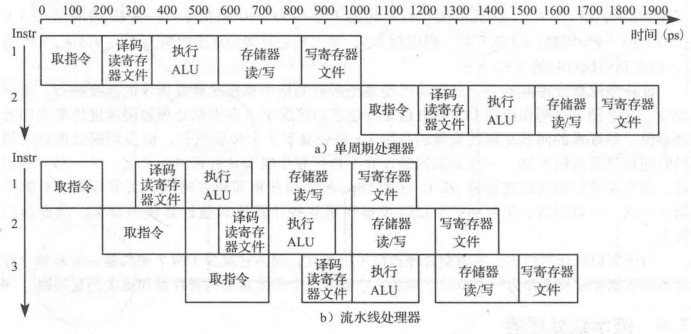
\includegraphics[width =0.95\linewidth]{figure/timestep.png}
\end{figure}

上图对比了单周期处理器与流水线处理器的时序图\footnote{图源于教材256页}。可以看出,流水线的吞吐量明显高于单周期,也说明了流水线处理器的高效性。

流水线系统中的核心问题是冲突(Hazard),即当后一条指令需要前一条指令的计算结果,而前一条指令还没有执行完时就会发生冲突。在这里,我们可以使用重定向、阻塞和刷新三种处理方法。

\newpage
\section{部件分析}

多周期处理器中大部分器件都与单周期相似,在此只列出新添加或发生改动的部件,其余请参考我的单周期报告。

\subsection{触发器flopr}

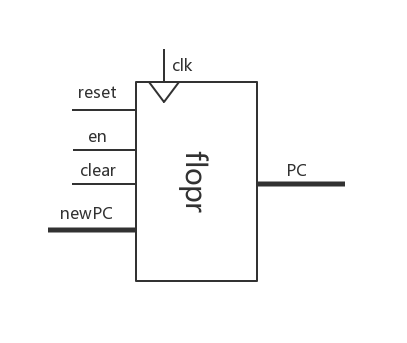
\includegraphics[width =0.35\linewidth]{figure/flopr.jpg}

流水线中,除了本来datapath中的寄存器,我们还需要添加两两阶段之间的状态寄存器。而为了支持状态的阻塞和刷新操作,我们需要给寄存器加入同步清零功能。所以,寄存器共有异步清零reset、使能en和同步清零clear三个控制口。

\subsection{比较器eqcmp}

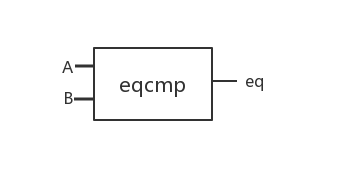
\includegraphics[width =0.3\linewidth]{figure/eqcmp.jpg}

为了提前预测beq和bne是否跳转,我们需要在decode阶段预判两个操作数是否相等,所以需要添加一个比较器。A与B都是32位数字,当A==B时,eq=1,当A!=B时,eq=0。


\subsection{数据通路Datapath}
\noindent
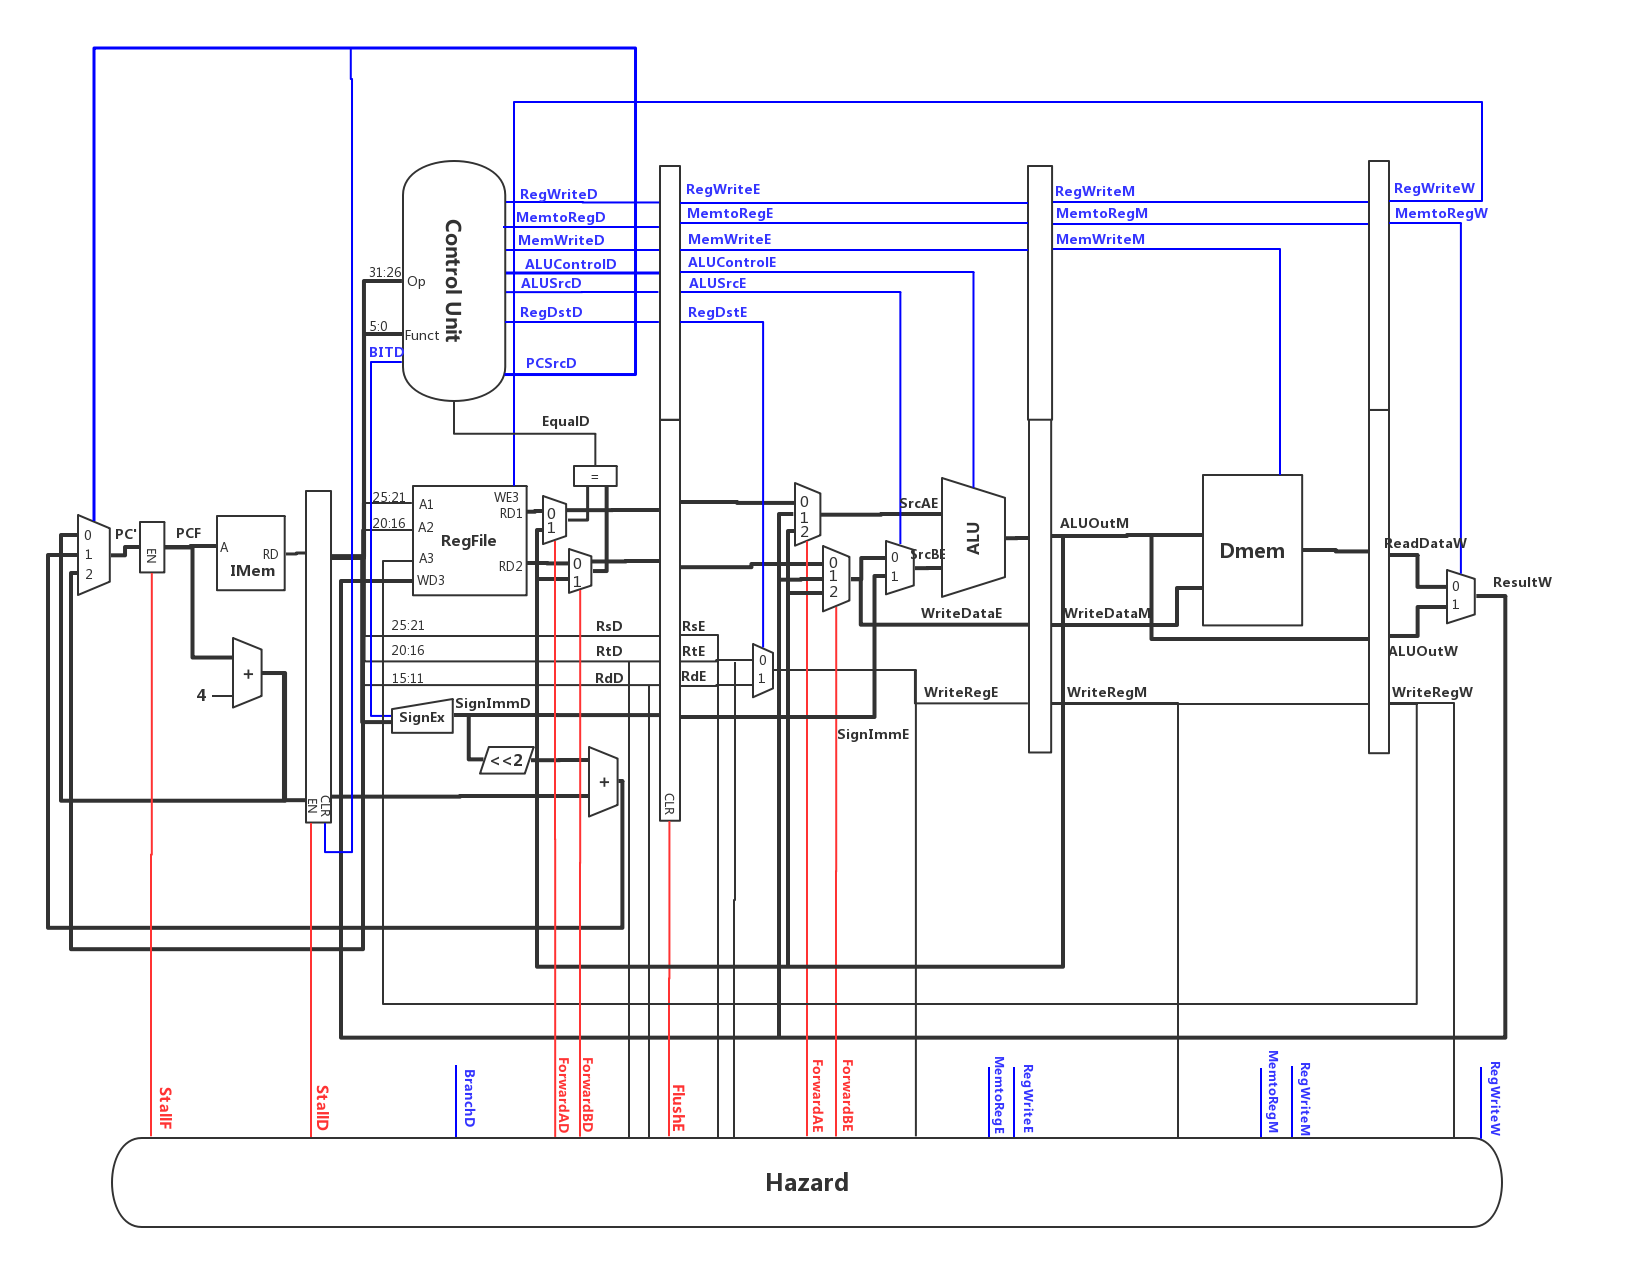
\includegraphics[width =\linewidth]{figure/Datapath.jpg}

{\bf 功能说明}:流水线数据通路与单周期相似,在单周期的结构上加入了状态寄存器,下面简单介绍一下结构。
\begin{itemize}
\item 左侧PC多路器,受PCSrcD和Jump信号控制,选择相应的PC值:信号为0时,选择下一条指令地址PC+4;信号为1时,选择D阶段计算出的相对寻址地址;信号为2时,选择指令中给出的绝对地址拼接PC高四位组成的地址。
\item 左侧PC寄存器,由StallF控制是否写入PC值,若StallF为1,则令F阶段暂停,不写入PC值。
\item 左侧Imem指令存储器,接受PC值作为输入地址,读出的指令传递给状态寄存器。
\item 左侧加法器计算PC+4的值,作为预测值传回PC多路器。
\item Decode阶段寄存器受StallD和PCSrcD(Jump)信号控制,分别控制其是否暂停和刷新,暂停时保持之前的状态,不写入新状态;刷新时,将当前阶段的状态清零。
\item 寄存器文件、位扩展、移位器、加法器作用都与单周期相似,在此略去。
\item Decode阶段增加了比较器,来比较从RegFile中取出的两个数是否相等,用于bne和beq指令的提前预测结果。
\item RegFile取出的两个数增加了转发逻辑,以应对数据冒险,将Memory阶段的计算值转发回来,以便用于相等判断。
\item Execute阶段状态寄存器中,需要接受解码出的控制信号、两个操作数、三个操作寄存器和位扩展后的立即数,由flushE信号控制是否刷新寄存器。
\item ALUSrcA和SrcB的参数直接由Execute的寄存器传入,加入转发逻辑,将Memory阶段与Writeback阶段计算出的信号传回,受信号ForwardAE与ForwardBE控制。
\item ALUSrcB的参数与单周期相似,可以是立即数,也可以是寄存器取出的值。
\item Memroy阶段状态寄存器中,存储ALU的计算结果,从寄存器中读取的需要写入内存的值,以及之后要进行写入的寄存器,还有几个控制信号。
\item Memory阶段与Writeback阶段功能结构基本与单周期相似,多出来的是加入了一些转发逻辑。
\end{itemize}

\subsection{控制模块Controller}

\subsubsection{控制信号说明}

控制信号有以下几种:
\begin{itemize}
\item {\bf RegWrite:} 控制是否写寄存器,会传递到Writeback阶段后作为RegFile的写使能。 
\item {\bf MemtoReg:} 是否是从Memory取数后写回到RegFile的指令,传递到Writeback阶段,选择返回的ResultW。
\item {\bf MemWrite:} 是否需要写内存,传递到Memory阶段后,作为Dmem的写使能信号。
\item {\bf ALUControl:} 选择ALU的运算,传递到Execute阶段后,接入ALU。
\item {\bf ALUSrc:} 选择ALUSrcB是寄存器值还是立即数,传递到Execute阶段。
\item {\bf RegDst:} 选择写入的寄存器,用于区分R型指令与I型指令,传递到Execute阶段选择完寄存器后,便可丢掉。
\item {\bf Branch:} 判断指令是否为beq,用于PCSrc的计算。
\item {\bf BNE:} 判断指令是否为bne,用于PCSrc的计算。
\item {\bf Jump:} 判断指令是否为j,用于PC来源的选择。
\item {\bf PCSrc:} 用于选择PC的来源,判断分支指令是否执行。若eqcmp结果为1且beq等于1,或eqcmp结果为0且bne等于1,则发生跳转,PCSrc=1。
\item {\bf BIT:} 判断位扩展时是采用符号扩展还是零扩展。
\end{itemize}

\subsubsection{实现细节}

控制模块的实现与单周期完全相同,可以直接copy过来。


\subsection{冲突处理模块Hazard}

本节主要介绍Hazard模块的信号逻辑设置,具体冒险的处理将在下一节中详细讨论。

Hazard模块接受控制信号、寄存器信息等等,返回控制信号,以控制整个流水线的转发逻辑、暂停和刷新逻辑,以此来应对冒险。输出的控制信号在图中已用红线标出,分为三种:Stall、Flush和Forward逻辑,分别对应暂停、刷新和转发,以下将介绍每种逻辑的控制。
\begin{itemize}
\item Decode阶段的转发信号ForwardAD与ForwardBD主要用于选择比较器的参数,因为Decode阶段中读的RegFile可能在之前的指令中已经被修改,但还未来得及写入寄存器中,所以这里需要引入转发逻辑,将Memory阶段的ALU结果转发回来。注意这里不能对Execute阶段的值转发,因为不一定来得及计算出来;同时,不需要对Writeback阶段的值进行转发,因为该值会在下降沿写入RegFile,在该时钟周期结束前,两个操作数的值就已变成正确的值了。信号的逻辑为,如果RegWriteM信号值为1,且写入的寄存器WriteRegM与相应的寄存器相同的话,则设置Forward信号为1。
\item Execute阶段的转发信号ForwardAE与ForwardBE主要用于选择ALU的参数。这两个参数是从寄存器文件中读出来的,而有可能该值已被前两条指令修改,但是在读的时候还未写入。这里的转发需要同时转发Memroy和Writeback阶段的值,所以信号的逻辑应为先判断RegWriteM是否为1和是否写入相应寄存器,再判断RegWriteW是否为1和是否写入相应寄存器。注意M的优先级高于W,因为M指令是后执行的。
\item 暂停和刷新的控制是一致的,即StallF、StallD与FlushE的控制逻辑相同。第一种情况是lw指令需要从内存中取值写入寄存器,因为在Memory阶段结束时才能取出值,所以无法进行转发。所以当Execute阶段的指令用到了在Memory阶段的lw指令的值时,需要插入一条nop指令,对应让Execute阶段刷新,Fetch和Decode阶段暂停。第二种情况是分支指令预测时,相应的寄存器值无法转发,必须要暂停一个周期,等寄存器值更新后再去判断。控制逻辑为,若控制信号BNE或Branch为1,且Execute阶段需要写入寄存器或Memory阶段为lw指令,并且写入寄存器与读的寄存器相同时,该信号为1。
\item Decode阶段寄存器的刷新信号由PCSrcD与Jump信号控制,当发现需要跳转时,我们之前取出的指令就需要作废了,所以刷新Decode寄存器避免该指令传递下去。
\end{itemize}


\newpage
\section{冲突处理与额外指令分析}

\subsection{额外指令分析}

因为时间就比较紧张,所以我在流水线阶段没有加入太多的指令。实际上,加入指令的逻辑并不复杂,且比较无聊,所以自己也就没有太大兴致继续加指令了。

\subsubsection{移位指令sll}

移位指令的加入主要是为了配合我的测试程序使用,有了移位指令,简单的乘法操作就可以实现了。加入的逻辑并不复杂,与多周期相同,直接把移位数传入ALU,并用ALUControl信号控制ALU运算即可。



\subsection{冲突处理}

冲突的分析与处理是流水线设计的难点。在流水线系统中,多条指令同时执行。当一条指令依赖于还没有结束的另一条指令的结果时,将发生冲突。冲突可分为{\em 数据冲突}和{\em 控制冲突}。当一条指令试图读取前一条指令还未写回的寄存器时将发生数据冲突。在取指令时还未确定下一条指令应取的地址时将发生控制冲突。

\subsubsection{利用转发(Forward)解决冲突}

当Execute阶段中的指令有一个与Memory阶段或Writeback阶段中的目的寄存器相匹配的源寄存器时,需要进行转发。一个典型的例子如下:
\begin{lstlisting}
0x0 : add $s0, $s2, $s3
0x4 : and $t0, $s0, $s1
0x8 : or  $t1, $s4, $s0
0xc : sub $t2, $s0, $s5
\end{lstlisting}
在or指令中源寄存器\$s0的值来源于add指令的计算结果,但是当or指令位于Decode阶段时,add指令还在Memory阶段,所以寄存器的值还没有被写入。所以当or指令进入Execute阶段后,需要通过转发逻辑将add指令的计算结果从Writeback转发过来。对于Memory阶段的数值也需要进行相似的转发操作。

\subsubsection{利用阻塞(Stall)解决冲突}

利用转发可以解决写后读(RAW)的冲突,但是lw指令知道存储器阶段后才能完成读数据,因此它的结果不能重定向到下一步指令的执行阶段。我们采取的解决方法是阻塞流水线,将操作挂起直至数据有效,等价于在Execute的阶段插入一条nop指令,同时使前面的指令暂停。一个典型的例子是:
\begin{lstlisting}
0x0 : lw  $s0, 40($0)
0x4 : and $t0, $s0, $s1
0x8 : or  $t1, $s4, $s0
0xc : sub $t2, $s0, $s5
\end{lstlisting}
这里and指令用到了lw指令中写入\$s0中的值,然而and在Decode阶段lw还没进行写入,and在Execute阶段时lw会在时钟周期结束时才能取出值,所以无法进行转发。这时的处理方法是让and指令等一个周期,在Execute中插入一条nop指令,同时让Decode阶段与Fetch阶段的指令暂停。

\subsubsection{解决控制冲突}

beq指令将产生控制冲突,因为在取下一条指令时分支是否发生还未确定,所以流水线处理器不知道取哪条指令。这里我们在Decode阶段加入比较器来预测分支跳转是否会发生。

糟糕的一条是,提前确定分支的硬件会产生新的RAW数据冲突。特别是,如果分支指令的一个源操作数由前一条指令计算得到且还没有写入寄存器文件,分支指令将从寄存器文件中读取错误的操作数值。我们可以通过前面使用的转发技术来解决数据冲突(如果可以进行转发),或者使用阻塞的方式,等到数据写入后再进行预测。

\subsubsection{一个糟糕的问题}

我在执行quick\_multiply.in这个样例时,发现了课本中提供的代码的错误。参考下面这个例子:
\begin{lstlisting}
0x10 : andi $t2, $t1, 1     | 312a0001
0x14 : beq $t2, $0, target  | 100a0001
0x18 : add $s0, $s0, $t0    | 02088020
0x1c : target:              | 
\end{lstlisting}
当beq指令进行预测时,其使用的操作数\$t2,在上一条指令中被修改,所以需要暂停,等待andi指令到Memory阶段进行转发。若此时\$t2的值恰好为0,那么就会出现FlushD(需要跳转,故刚刚读出的指令不向下传递)与StallD(暂停,等待andi指令计算完)同时为1的情况,此时,我们应该选择刷新还是暂停呢?课本中直接将两个信号同时传入,因为在寄存器的设计中刷新的优先级较高,所以会将该指令刷新掉。与此同时,Fetch阶段暂停了,Execute阶段刷新了,所以这条beq指令就凭空消失了,当真的需要执行跳转分支时,也不会执行,所以会出现错误。

正确的处理方式是在传入flushD信号时,保证二者不会同时为1,即传入以~stallD \& flushD信号传入。这样当stallD为1时,flushD就永远不会为1。那么,为什么我们不直接在寄存器中设置写使能的优先级高于清零呢?因为如果写使能优先级始终较高的话,对于一些写使能恒为1的寄存器,就无法执行刷新操作了。当然,也可以为它单独设计一个寄存器。不过相比之下,强制让信号互斥是更好的处理方案。


\newpage
\section{测试样例与结果}

与单周期相同的测试样例均已通过,这里只列举几个关键的和新加入的测试样例。

\subsection{all.in}

\begin{lstlisting}
 0x0 : addi $s0, $0, 12     | 2010000c
 0x4 : andi $s2, $s0, -8    | 3212fff8
 0x8 : ori $s3, $s1, 10     | 3633000a
 0xc : slti $s4, $s2, 5     | 2a540005
0x10 : nop                  | 00000000
0x14 : add $t0, $s0, $s1    | 02114020
0x18 : sub $t0, $s2, $s3    | 02534022
0x1c : and $t0, $s3, $s1    | 02714024
0x20 : or $t0, $s1, $s2     | 02324025
0x24 : slt $t0, $s0, $s2    | 0212402a
0x28 : sw $s0, 0($0)        | ac100000
0x2c : lw $t0, 0($0)        | 8c080000
0x30 : nop                  | 00000000
0x34 : nop                  | 
\end{lstlisting} 

注意,这里需要在所有指令结束后添加nop指令,因为当最后一条指令在存储器和写回阶段时,流水线需要有可以读取的指令。测试结果如下:

\noindent
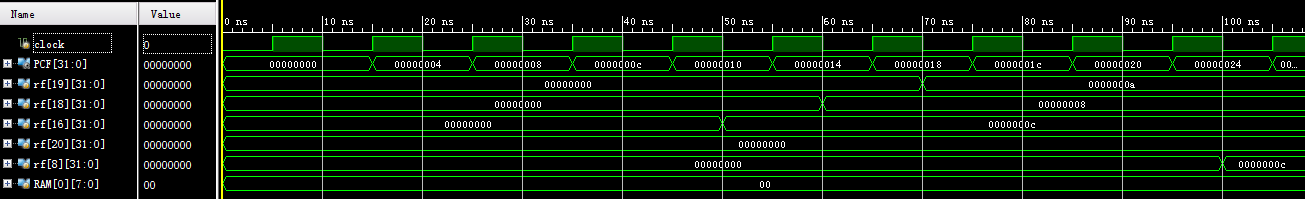
\includegraphics[width =\linewidth]{figure/all1.png}
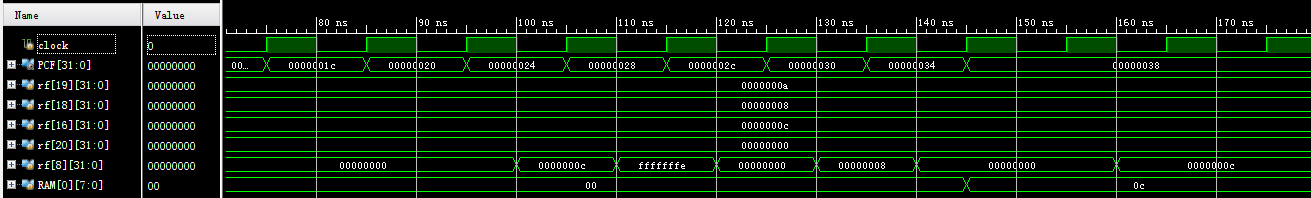
\includegraphics[width =\linewidth]{figure/all2.png}

上图中依次给出了寄存器 \$s3, \$s2, \$s0, \$s4 和 \$t0,以及内存地址0处的值。每条指令的结果依次应为:

\$s0 = 12 $\rightarrow$
\$s2 = 8 $\rightarrow$
\$s3 = 10 $\rightarrow$
\$s4 = 0 $\rightarrow$
nop $\rightarrow$
\$t0 = 12 $\rightarrow$
\$t0 = -2 $\rightarrow$
\$t0 = 0 $\rightarrow$
\$t0 = 8 $\rightarrow$
\$t0 = 0 $\rightarrow$
0(\$0) = 12 $\rightarrow$
\$t0 = 12


\subsection{gcd.in}

\begin{lstlisting}
 0x0 : addi $v0,$0,189      | 200200bd
 0x4 : addi $v1,$0,287      | 2003011f
 0x8 : main:                | 
 0x8 : beq $v0,$v1,end      | 10620007
 0xc : slt $at,$v0,$v1      | 0043082a
0x10 : beq $at,$0,run       | 10010003
0x14 : add $at,$v0,$0       | 00400820
0x18 : add $v0,$v1,$0       | 00601020
0x1c : add $v1,$at,$0       | 00201820
0x20 : run:                 | 
0x20 : sub $v0,$v0,$v1      | 00431022
0x24 : j main               | 08000002
0x28 : end:                 | 
0x28 : add $t3, $0, $0      | 00005820

\end{lstlisting}

这个测试样例是从黄文皓同学那里借来的,通过循环计算两个数的最大公约数。开始时,我们把需要计算的两个数字189和287分别赋值给\$v0和\$v1。之后,通过辗转相减法计算最大公约数。当\$v0与\$v1相等时,说明计算得到了它们的最大公约数。

\noindent
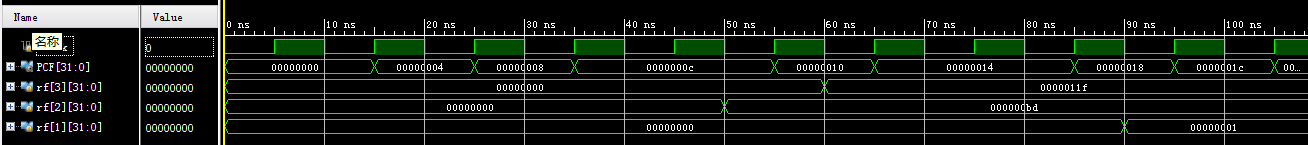
\includegraphics[width =\linewidth]{figure/gcd1.png}
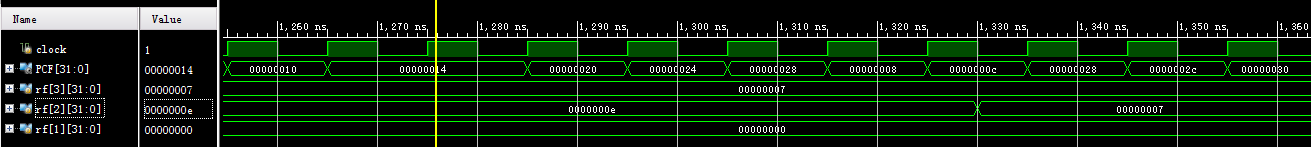
\includegraphics[width =\linewidth]{figure/gcd2.png}

这里的两幅图分别展示了程序开始与结束时的计算结果。从第一幅图可以看到程序正常的执行循环,后一幅图则说明程序成功地计算出两数的最大公约数为7。


\subsection{quick\_multiply.in}

\begin{lstlisting}
 0x0 : addi $t0, $0, 99     | 20080063
 0x4 : addi $t1, $0, 37     | 20090025
 0x8 : addi $s0, $0, 0      | 20100000
 0xc :                      | 
 0xc : while:               | 
 0xc : beq $t1, $0, done    | 10090006
0x10 : andi $t2, $t1, 1     | 312a0001
0x14 : beq $t2, $0, target  | 100a0001
0x18 : add $s0, $s0, $t0    | 02088020
0x1c : target:              | 
0x1c : sll $t0, $t0, 1      | 00084040
0x20 : srl $t1, $t1, 1      | 00094842
0x24 : j while              | 08000003
0x28 :                      | 
0x28 : done:                | 
0x28 : add $t3, $0, $0      | 00005820
\end{lstlisting} 

这个代码曾在单周期处理器中演示过,用于计算两数的乘积,方法类似快速幂。首先将99与37写入\$t0和\$t1寄存器,然后进入循环,每次根据\$t1的末位是否为1,来决定是否向\$s0进行累加,然后每次\$t0乘2,\$t1右移一位。最终,计算结果存在\$s0中,应为0xe4f。这个测试样例测试了跳转、移位等指令,测试结果如下:

\noindent
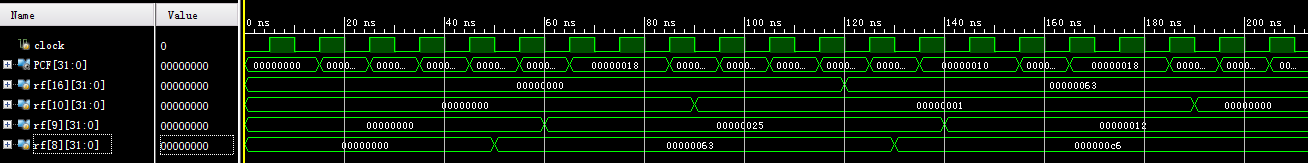
\includegraphics[width =\linewidth]{figure/mul1.png}
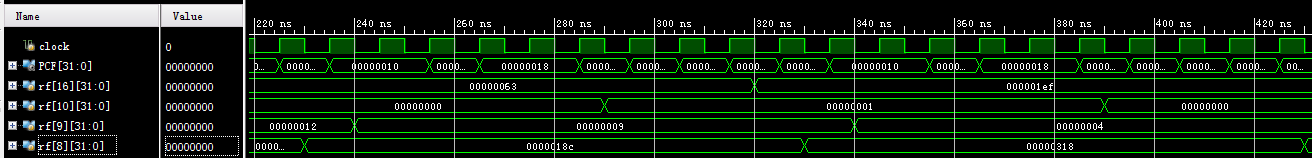
\includegraphics[width =\linewidth]{figure/mul2.png}
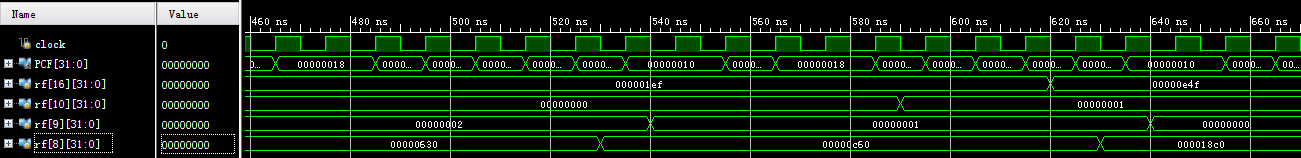
\includegraphics[width =\linewidth]{figure/mul3.png}

图中依次展示的是寄存器\$s0,\$t2,\$t1,\$t0的值,可以看到程序开始时,寄存器\$t0与\$t1分别被赋值为0x63与0x25,分别对应99与37。循环过程中,\$t0每次乘2,\$t1每次除以2,最终\$s0变为0xe4f,结果正确,说明程序正确执行。



\section{注意事项}

\subsection{遇到的问题}

\begin{enumerate}
\item 寄存器文件要设置为下降沿写入。
\item 不要迷信书上的代码,书上的代码也会有错。
\item 使用未定义的变量,Verilog是不会报错的,但是在仿真的时候会出现奇怪的数值,所以写完代码后一定要仔细检查变量名与连线。
\end{enumerate}

\section{申A理由}

\begin{itemize}
\item 实现了所有的基本指令
\item 首先发现了书中代码的bug,并帮助其他人解决了这个问题
\item 自己动手画图来描绘流水线的结构(见Datapath)
\end{itemize}

\end{sloppypar}
\end{document}
